\subsection{System Topologie}
\begin{figure}[H]
\centering
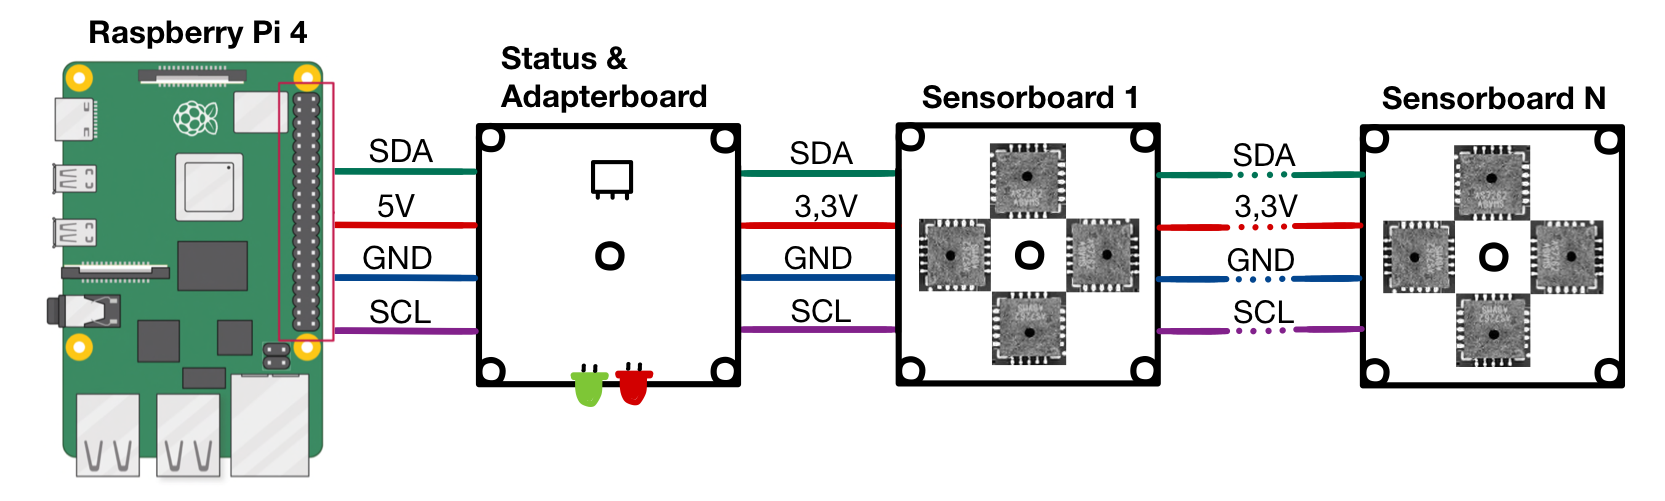
\includegraphics[width=1\textwidth]{img/System-Topologie.png}
\caption{Verschaltung der der Platienen \cite{Pi_4_Top_view}}
\label{fig:Verschaltung_der_P}
\end{figure}

Der Messaufbau besteht aus einem Rapberry Pi 4 Model B welcher über eine Status und Adapterplatinene mit 1-10 Sensnorboards verbunden werden kann (Abbildung \ref{fig:Verschaltung_der_P}).


\subsection{Status \& Adapterboard}
Da wie in Abschnitt \ref{Mikrocontroller} erklärt der Rapberry Pi nicht die benötigte 3,3V Stromversorgung bereitstellt wird eine Adapterboard (Abbildung \ref{fig:Adapter-Shield}) mit einem Spannungswandler (LM3940IT-3.3) verwendet.
Auf dem Adapterboard findet der einheitliche Steckverbinder sowie die Pull Up widerstände des I2C Bus Platz, da das Adapterboard aufgrund seiner Bauform nicht falsch montiert werden kann so die Verpolung der Sensoren ausgeschlossen werden.
Die Bedeutung der Status LED wird im Handbuch unter Abschnitt \ref{leds} erläutert.\\ 
Der überflüssige Platz auf dem Adapterboard wurde für einen Prototyping-Bereich genutzt.

\begin{figure}[H]
\centering
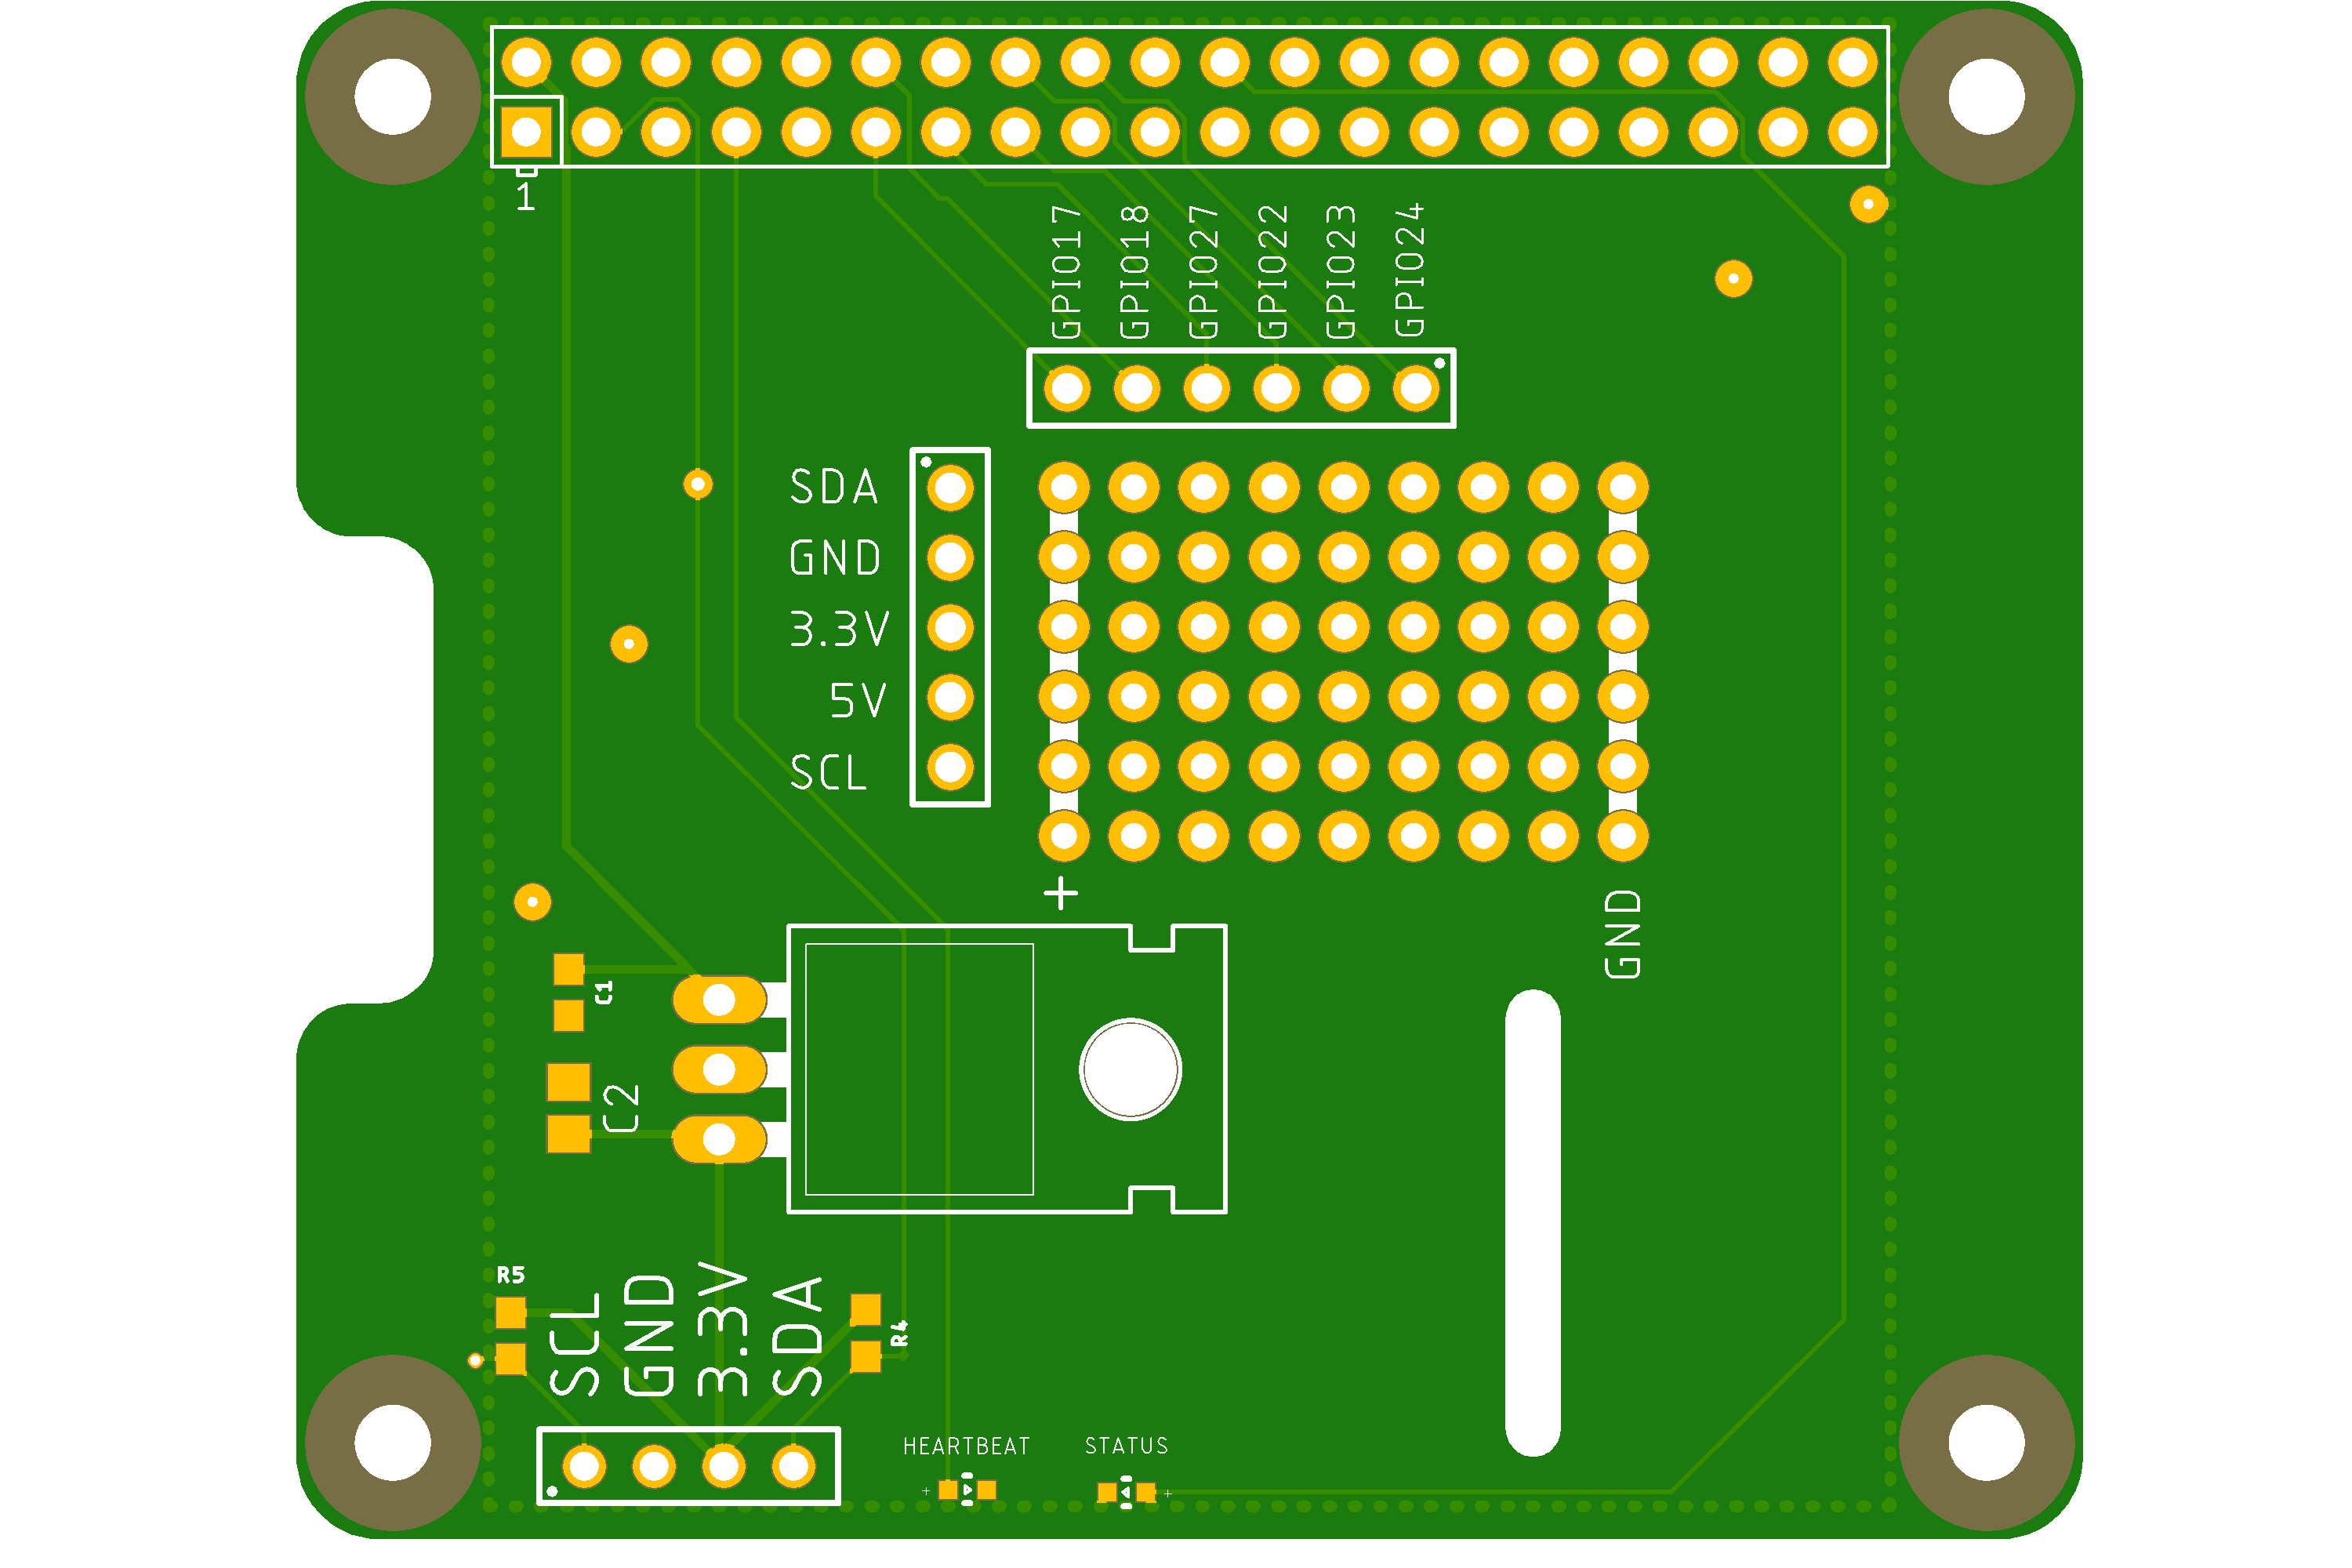
\includegraphics[width=0.8\textwidth]{img/pi-shield}
%\caption*{Quelle: Datenblatt AS7261}
\caption{Platine des Status \& Adapterboard}
\label{fig:Adapter-Shield}
\end{figure}
\subsection{Sensorboard}
Die Hauptaufgabe der Sensorboard Platine ist es den AS7261 und der AS7265X mit ihrem Companion Flash (Abschnitt \ref{sec_Companion_Flash}) und über den I2C Translator (Abschnitt \ref{I2C-Translator}) dem I2C Bus zu verbunden.
Außerdem werden verschiedene benötigte LEDs, Wiederstände und Kondensatoren verbaut.


\paragraph{Status LED:} Am AS7261 und AS7265X Befindet sich je­weils eine Rote Status LED wenn es ein Problem mit dem Companion Flash gibt fängt sie an zu blinken im normalbetrieb kann die LED Softwareseitig ein und ausgeschaltet werden.
	Während der Messung sollte sie ausgeschaltet werden da das rote Licht sonst die Messung verfälscht.

\paragraph{Pull-up-Widerstände:}
R7 und R8 sind die Pullup Widerstände des seperaten I2C Bus welcher die AS7265X Sensoren miteinander verbindet.\\
R12 und R11 sind die Pullup Widerstände des I2C Bus welcher den AS7261 mit seinem LCT4316 verbindet.\\
R4 und R5 sind die Pullup Widerstände des I2C Bus welcher den AS72651 mit seinem LCT4316 verbindet.

\paragraph{I2C Enable Wiederstände:} Pin R6 ist mit 3.3V und Pin 8 (I2C Enable) des AS7261 verbunden. So wird 
I2C als Kommunikationsmodus des AS7261 ausgewählt.
	R3 erfüllt die gleiche Aufgabe für den AS72651.
	
\paragraph{Translation Byte Wiederstände:}
Die 8 Wiederstände auf der Rückseite R1\_XX und R2\_XX sind die in \ref{I2C-Translator} beschriebenen Wiederstände welche das Translation Byte einstellen. Die Wiederstände R1\_XX bestimmen die Addresse des AS7261 und R2\_XX die Addresse des AS72651.

\paragraph{Entstörkondensatoren:} Im Datenblatt der Sensoren wird empfohlen, für jeden Sensor 2 Parallele Entstörkondensatoren mit den Kapazitäten $10uF$ und $100nF$ so nah wie möglich am Sensor zwischen GND und VCC zu platzieren.


\begin{center}
\begin{tabular}{ c c c }
 Kürzel & Wert & Sensor \\ 
 C5 & $10uF$ & AS7261 \\  
 C4 & $100nF$ & AS7261 \\
 C1 & $10uF$ & AS72651 \\  
 C8 & $100nF$ & AS72651 \\
 C2 & $10uF$ & AS72652 \\  
 C3 & $100nF$ & AS72652 \\
 C7 & $10uF$ & AS72653 \\  
 C6 & $100nF$ & AS72653 \\
\end{tabular}
\end{center}

\begin{figure}[H]
\centering
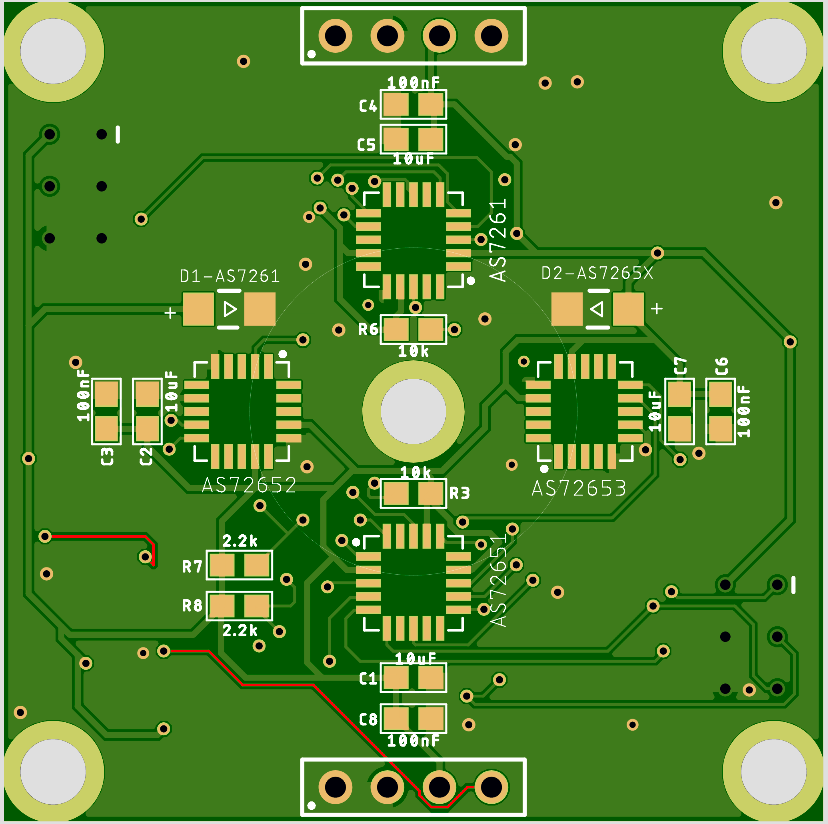
\includegraphics[width=0.75\textwidth]{img/Sensor-platiene_front}
%\caption*{Quelle: Datenblatt AS7261}
\caption{Vorderseite des Sensorboards I2C Leitungsverlauf in Rot}
\label{fig:Sensor-platiene_front}
\end{figure}

\begin{figure}[H]
\centering
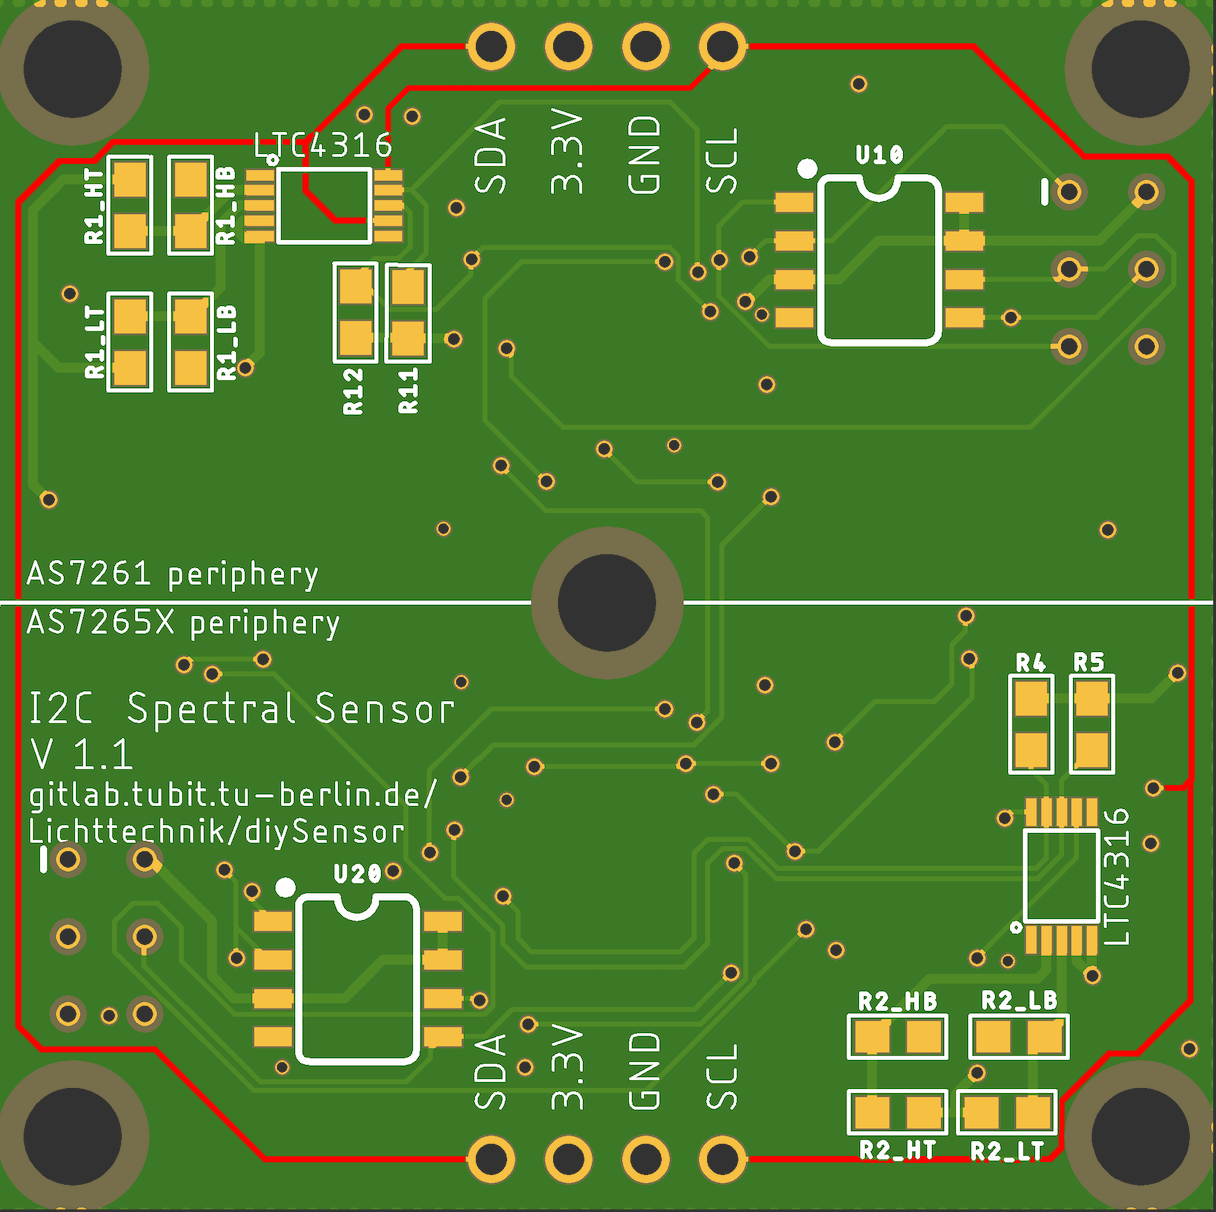
\includegraphics[width=0.75\textwidth]{img/Sensor-platiene_back}
%\caption*{Quelle: Datenblatt AS7261}
\caption{Rückseite des Sensorboards I2C Leitungsverlauf in Rot}
\label{fig:Sensor-platiene_back}
\end{figure}

\paragraph{I2C Lanes:}
Die I2C Leitungen haben ihren Ursprung auf der Adapterplatine und werden mithilfe der seitlichen Steckverbinder über die Sensorboards durchgeschleift.
Die maximal mögliche Länge einer I2C Leitung hängt von der Länge der Leitungskapazität sowie äußeren Störeinflüssen ab.
Die Data und die Clock Leitung sind möglichst weit von anderen Datenleitungen, also auch von einander entfernt platziert, da so Störeinflüsse durch elektromagnetische Felder minimiert werden.
Außerdem wurde darauf geachtet, das die beiden Leitungen auf den Platinen die gleiche Länge habe da sich sonst die Differenzen der Leitungslänge mit jeder angeschlossenen Platine addiert und es zu Timing Differenzen zwischen der Daten und Clock Leitung kommt.
Der Verlauf der Leitungen ist in Abbildung \ref{fig:Sensor-platiene_back} und \ref{fig:Sensor-platiene_front} Rot gekennzeichnet.

\paragraph{Connector:} Es gibt 4 durchkontaktierte Löcher auf der rechten und linken Seite der Platine, hier können unterschiedliche Steckverbinder mit 2.54 mm Pitch montiert werden.
	Es empfiehlt sich, verpolungssichere Steckverbinder zu verwenden, um Hardware Schäden vorzubeugen.
	Für dieses Bauteil wurde keine SMD-Technik, sondern Durchsteckmontage gewählt, da so eine bessere mechanische Festigkeit erreicht wird.
	Außerdem kann so alternativ zu einem Steckverbinder direkt ein Flachbandkabel angelötet werden.

